\section{Self Study 1: Preliminary Database Modeling}
\deadline{12}{2}{2014}

As stated in the assignment, we have decided to look at different possible attributes and models by looking at the structure of movie pages on IMDB\@. Initially, we think it would require many join tables, as we've identified a few many-to-many relationships among structures we've discussed. These structures are: \emph{actors}, \emph{directors}, \emph{writers}, \emph{movies}, \emph{awards}, \emph{ratings}, and \emph{users}.

\begin{figure}[H]
  \centering
  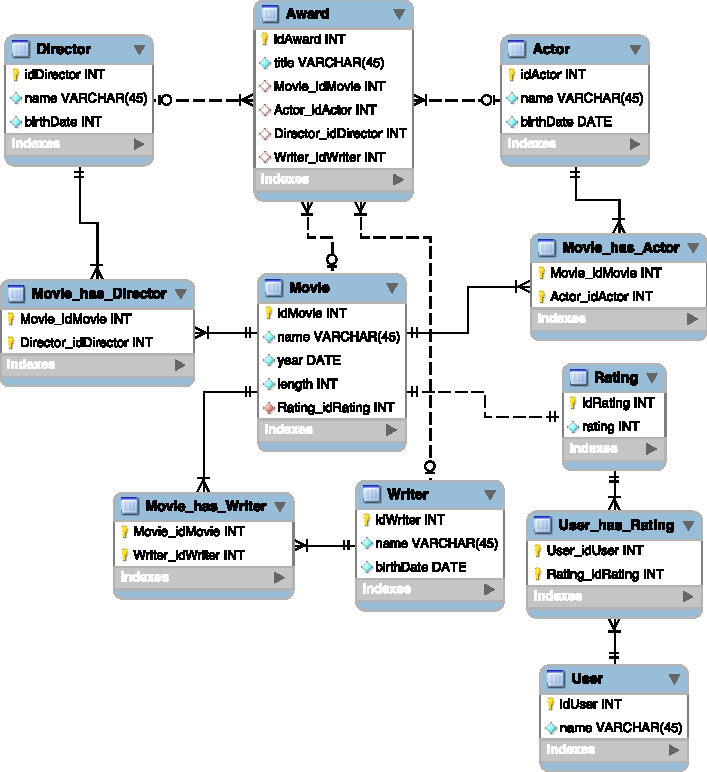
\includegraphics[width=\linewidth]{1-06.02.14/selfStudy1db.pdf}
  \caption{Enhanced entity-relationship (EER) model diagram of a simplified movie database.}\label{fig:model}
\end{figure}

We spent time on figuring out how to map the relationships between tables
instead of focusing on the attributes. In our opinion it is easy to just add a
birthdate if that should be necessary.

Figure \ref{fig:model} shows relationships between the chosen models and their
corresponding join tables. Dashed lines between tables repressent
\emph{non-identifying} relationships and
solid lines between tables represent \emph{identifying} relationships.

When lines branch toward a table then there is a ``has many'' relationship to
that table. When the lines have two orthogonal dashes (or a orthogonal dash and
a circle) by a table then there is a
``has one'' relationship to that table. If there is a circle then the
relationship is non-identifying.
For example one \emph{Director} has many \emph{Awards}. The relationship is
also non-identifying because the tables can exist indenpendently of each other.

The SQL for creating this structure is presented in see section \ref{sec:sqlPre}.


